\documentclass[a4paper, 12pt, openany, oneside]{book}
% Header file
% author: marcobecerrap
% date: January-2015

\usepackage{cite} % Citation Package
\usepackage{natbib} % Citation style
\usepackage{graphicx} % Graphics Package
\usepackage{amssymb, amsmath, amsbsy} % Equations
\usepackage{caption}
\usepackage{subcaption}
%\usepackage[utf8]{inputenc} % Special characters (e.g. spanish accents).
\usepackage{pgfgantt} % Gantt Charts
\usepackage{lscape} % Included packages located in a separate file
\pagestyle{plain} %Page numbers on the bottom

\begin{document}

% Front page
\pagestyle{emty} %No numbers
%\begin{titlepage}
%\begin{center}
%	{UoB, CS}\\
%	{Report 3}\\
%	{Title: SM of HE with a MR}\\
%	{Student: MABP}\\
%	{Supervisor: NH}\\
%	{Thesis Group: JW PH}
%\end{center}
%\end{titlepage}


\begin{titlepage}
\begin{center}

   {\Large \textsc{University of Birmingham}}
	\vskip 10pt
	{\Large \sc School of Computer Science}

%\vskip 0pt plus 2fill
\vspace{50pt}
{\Huge\bf Thesis proposal }\\
\vspace{40pt}
\includegraphics[width=6cm]{fig/uob_coat.pdf}
%\pgfdeclareimage[width=8.5cm]{logo}{fig/logo_cvut}
%\pgfuseimage{logo}

\vspace{40pt}
{\Large\rm Marco Antonio Becerra Pedraza} \\
\vspace{20pt}
{\Large\bf Semantic Mapping of Human Activities}\\
\vspace{0.2cm}
{\Large\bf with a Mobile Robot}\\

\vspace{40pt}
{\bf Intelligent Robotics Lab}\\
\vspace{5pt}   
{Supervisor: {\bf Dr. Nick Hawes}}\\
\vspace{5pt}   
{Thesis group members: {\bf Prof. Jeremy Wyatt, Dr. Peter Hancox}}
\vfill 
{Birmingham, 26.3.2015}
\end{center}
\end{titlepage}
\cleardoublepage

% Table of Contents
\newpage
\pagenumbering{roman}
\tableofcontents

% Main Chapters
\newpage
\pagestyle{plain}
\pagenumbering{arabic}
% Abstract
%\chapter{Introduction}

% INTRO 
% > Robots in everyday environments are important.
% > This environment is hard.
% > Robots needs cognitive skills: understand the environment.
\section{Introduction}
One of the main goals in AI is having robots working autonomously in everyday environments. 
In such situation, robots are expected to perceive, understand and interact with its environment. 
However, these kind of environments are dynamic, non-structured and non-deterministic, which makes difficult for a robot to fulfil the assigned tasks. 
To be able to sort these obstacles, robots need to be provided with cognitive skills.

Human cognition refers to all mental activities associated with thinking, knowing, remembering and communicating, and how the information is processed \citep{King2014Psychology,myers2013psychology}. 
In robotics, the concept is associated with systems that emulate these mental processes or those that \textit{sense}, \textit{plan} and \textit{act}.
More precisely, cognition can refer to those systems that can perceive, understand \ldots and interact with their environment, and evolve in order to achieve human-like performance in activities requiring context (situation and task) specific knowledge \citep{christensen2010cognitive}.

% GENERALITIES ABOUT HUMAN ACTIVITIES
% > Activities are important part of the scenes and they are necessary to be able to understand the scene
% > Activities are entities with a spatio-temporal & symbolic (semantic, hierarchical) characteristics
Everyday environments have many valuable features that a robot needs to understand, in order to succeed while performing a task, among them are human activities.
Human activities are a meaningful manifestation of human behaviour along time and space. %TODO Expand the definition of activity.
They provide rich information about the human performing it, but also, about his/her relation with other relevant components of the environment as humans, objects and locations.


%\section{Research Problem}
\subsection{Human activity analysis with a mobile robot}
% ACTIVITY RECOGNITION
% > AR as a field
% > Robot case, advantages and disadvantages of using a robot
Activity recognition is the research field that studies the automatic detection and analysis of human activities by processing the data acquired from sensors \citep{Aggarwal14_HumActRec3DRev}. 
It is not restricted only to sensory data and this can also be complemented with other sources of information, i.e. domain knowledge.
In the AI context, activity recognition is closely related with the areas of perception, knowledge representation and reasoning. 
The problem of activity recognition has been treated from different perspectives, however, computer vision has been the most popular.

% Robots in AR (general)
In principle, robots with appropriate sensing and processing capabilities can perform activity recognition. 
Moreover, they have some advantages over the use of fixed cameras or wearable devices as they are able to interact with the environment. 
Robots are active observers, i.e. they can change their point of view on scene and be selective in the areas of the environment that are more interesting. 
On the other hand, they have some disadvantages as well. 
They don't have omnipresence, so they are not able to sense the full environment and will loose information.
Also, their sensors have constraints, the data may be noisy or blurry due to movement, erratic hardware, changing environmental conditions, etc. 
Finally, robots are expected to work in real-time, so online activity recognition is desirable but yet difficult to achieve.

% BRIDGE TO ASP
Activities involve knowledge.
They associate concepts and relations between a subject and the environment.
In general, an activity recognition system should be able to handle, not only sensory data but also symbolic representations, and be able link top level symbolic concepts to low level sensory data; this is known as the \textit{anchoring problem} \citep{Coradeschi03_AnchoringProblem}.
With this in mind, knowledge processing and reasoning is a necessity for such systems.


\subsection{Answer Set Programming for Knowledge Representation and Reasoning}

There have been proposed many ideas to handle the problems of knowledge representation and reasoning (e.g. logic programming, ontologies, bayesian networks, fuzzy logic, etc.), among them is Answer Set Programming (ASP).
ASP is form of declarative programming oriented towards difficult, primary NP-hard, search problems.
It establish a new paradigm of logic programming that allows concepts as negation as a failure, default knowledge and non-monotonic reasoning.

ASP main concepts were proposed since the late 1980s \citep{Gelf88a} and it has been used with success in many applications.
Traditionally, ASP solvers were designed as one-shot problem solvers, so they lacked of reactive capabilities and, for example, whenever new data arrived, the system needed to be restarted.
This has been one of the main reasons why ASP has not been fully exploited in the field of robotics, however, in recent years an important effort has been directed towards this direction by some groups \citep{AndresOSSR13_rosoclingo,Erdem2013_IntLowRTaskP}.


\section{Research Problem}

This project is based in the consideration of ASP as a solid option for robots in problems that require symbolic representations.
The focus of this project is to study \textbf{ASP-based activity recognition with a mobile robot}. The interest lies  in the spatio-temporal relation between human activities and the environment and how a robot can acquire, handle and use this knowledge.

ASP allows the manipulation of incomplete information and handling multiple sources of knowledge.
The integration between observations and external knowledge appear to be a more robust approach than a single sensory based approach.
Hardware adds uncertainty via noise, is constrained by its specification and the outcome data is usually difficult to process.
This uncertainty cannot be eradicated in robots, but the treatment of some problems as activity recognition can be boosted by emphasizing a more cognitive approach. 
%(via) the it can be  by emphasizing cognitive mechanisms By putting emphasis in the cognitive essence of the problem of activity recognition, the uncertainty in the cognitionemphasizing aputting emphasis in athe upper layer of knowledge representation and reasoning in solving problems that require cognition, the system would rely totally onenable, not to eradicate, but to complement a sensory based approach and also to minimize its charge in a system.

\subsection{Expected outcome}

The expected outcome will be a systematic analysis of ASP-based activity recognition and its use with a mobile robotic platform.

First, the problem of activity recognition will be treated via ASP and compared with other state-of-the-art approaches.

Experience acquisition will be studied via semantic mapping to progressively create a knowledge source for a robot regarding the activities occurring in a particular location and that can be used by the robot for future inferences.

Finally, we are interested in taking advantage of the activeness of the robot to improve the perception and knowledge acquisition processes in the context of activity recognition; e.g. looking for missing information, the ability to get information from the environment more efficiently, etc.



% RESEARCH PROBLEM
% > Talk about AR with a robot in cases with incomplete information
% > Generalities of the problem 
% > Example case of a sequence
%TODO %TODO %TODO %TODO %TODO %TODO %TODO %TODO %TODO %TODO %TODO %TODO %TODO %TODO %TODO %TODO

%Persentation of the project
%Particularly in the case where there is not complete information from the environment to have a clear match between the observations and %the activity patterns. 
%Here, an interpretation can still be made using previous experience and domain knowledge. 
%Even, if a totally certain interpretation of the scene is not possible, a partial one can still be done with a list of the most probable situations to be happening. 
%This also can be used by a robot to decide to perform new observations of the scene to improve its reasoning conclusions. 
%The chosen technique to do this is Answer Set Programming (ASP).

%TODO Write paragraph about ASP
%Answer Set Programming is a logical p

% Quick draft of the proposal.

\section{Test scenario: ``The library setting''} \label{sec_Library} %TODO Add images.

Because human activities cover a broad range o possible situations, it becomes a necessity to bound the scope of this project and look into exemplar cases that can be used to demonstrate the ideas. 
With this in mind, it has been chosen a library as a scenario to test and explain the ideas of this project.

The School of Computer Science at the University of Birmingham has a library, Fig. \ref{fig_library}.
The physical scenario is basically a big room. 
It has some cabinets (where bibliographic material is stored), a reception desk, some tables with chairs and a printing area. 
It has only one entrance.
An attendant is in charge of the book loans and retrievals, and also to assist the users.
Most users use the facility to study, to consult material, to print, for team work, to use their laptops or simply as a rest area.

%TODO Add images (1) real library, (2) Lars SemMap
\begin{figure}[tbp]
  \centering
  \subfloat[Real library]{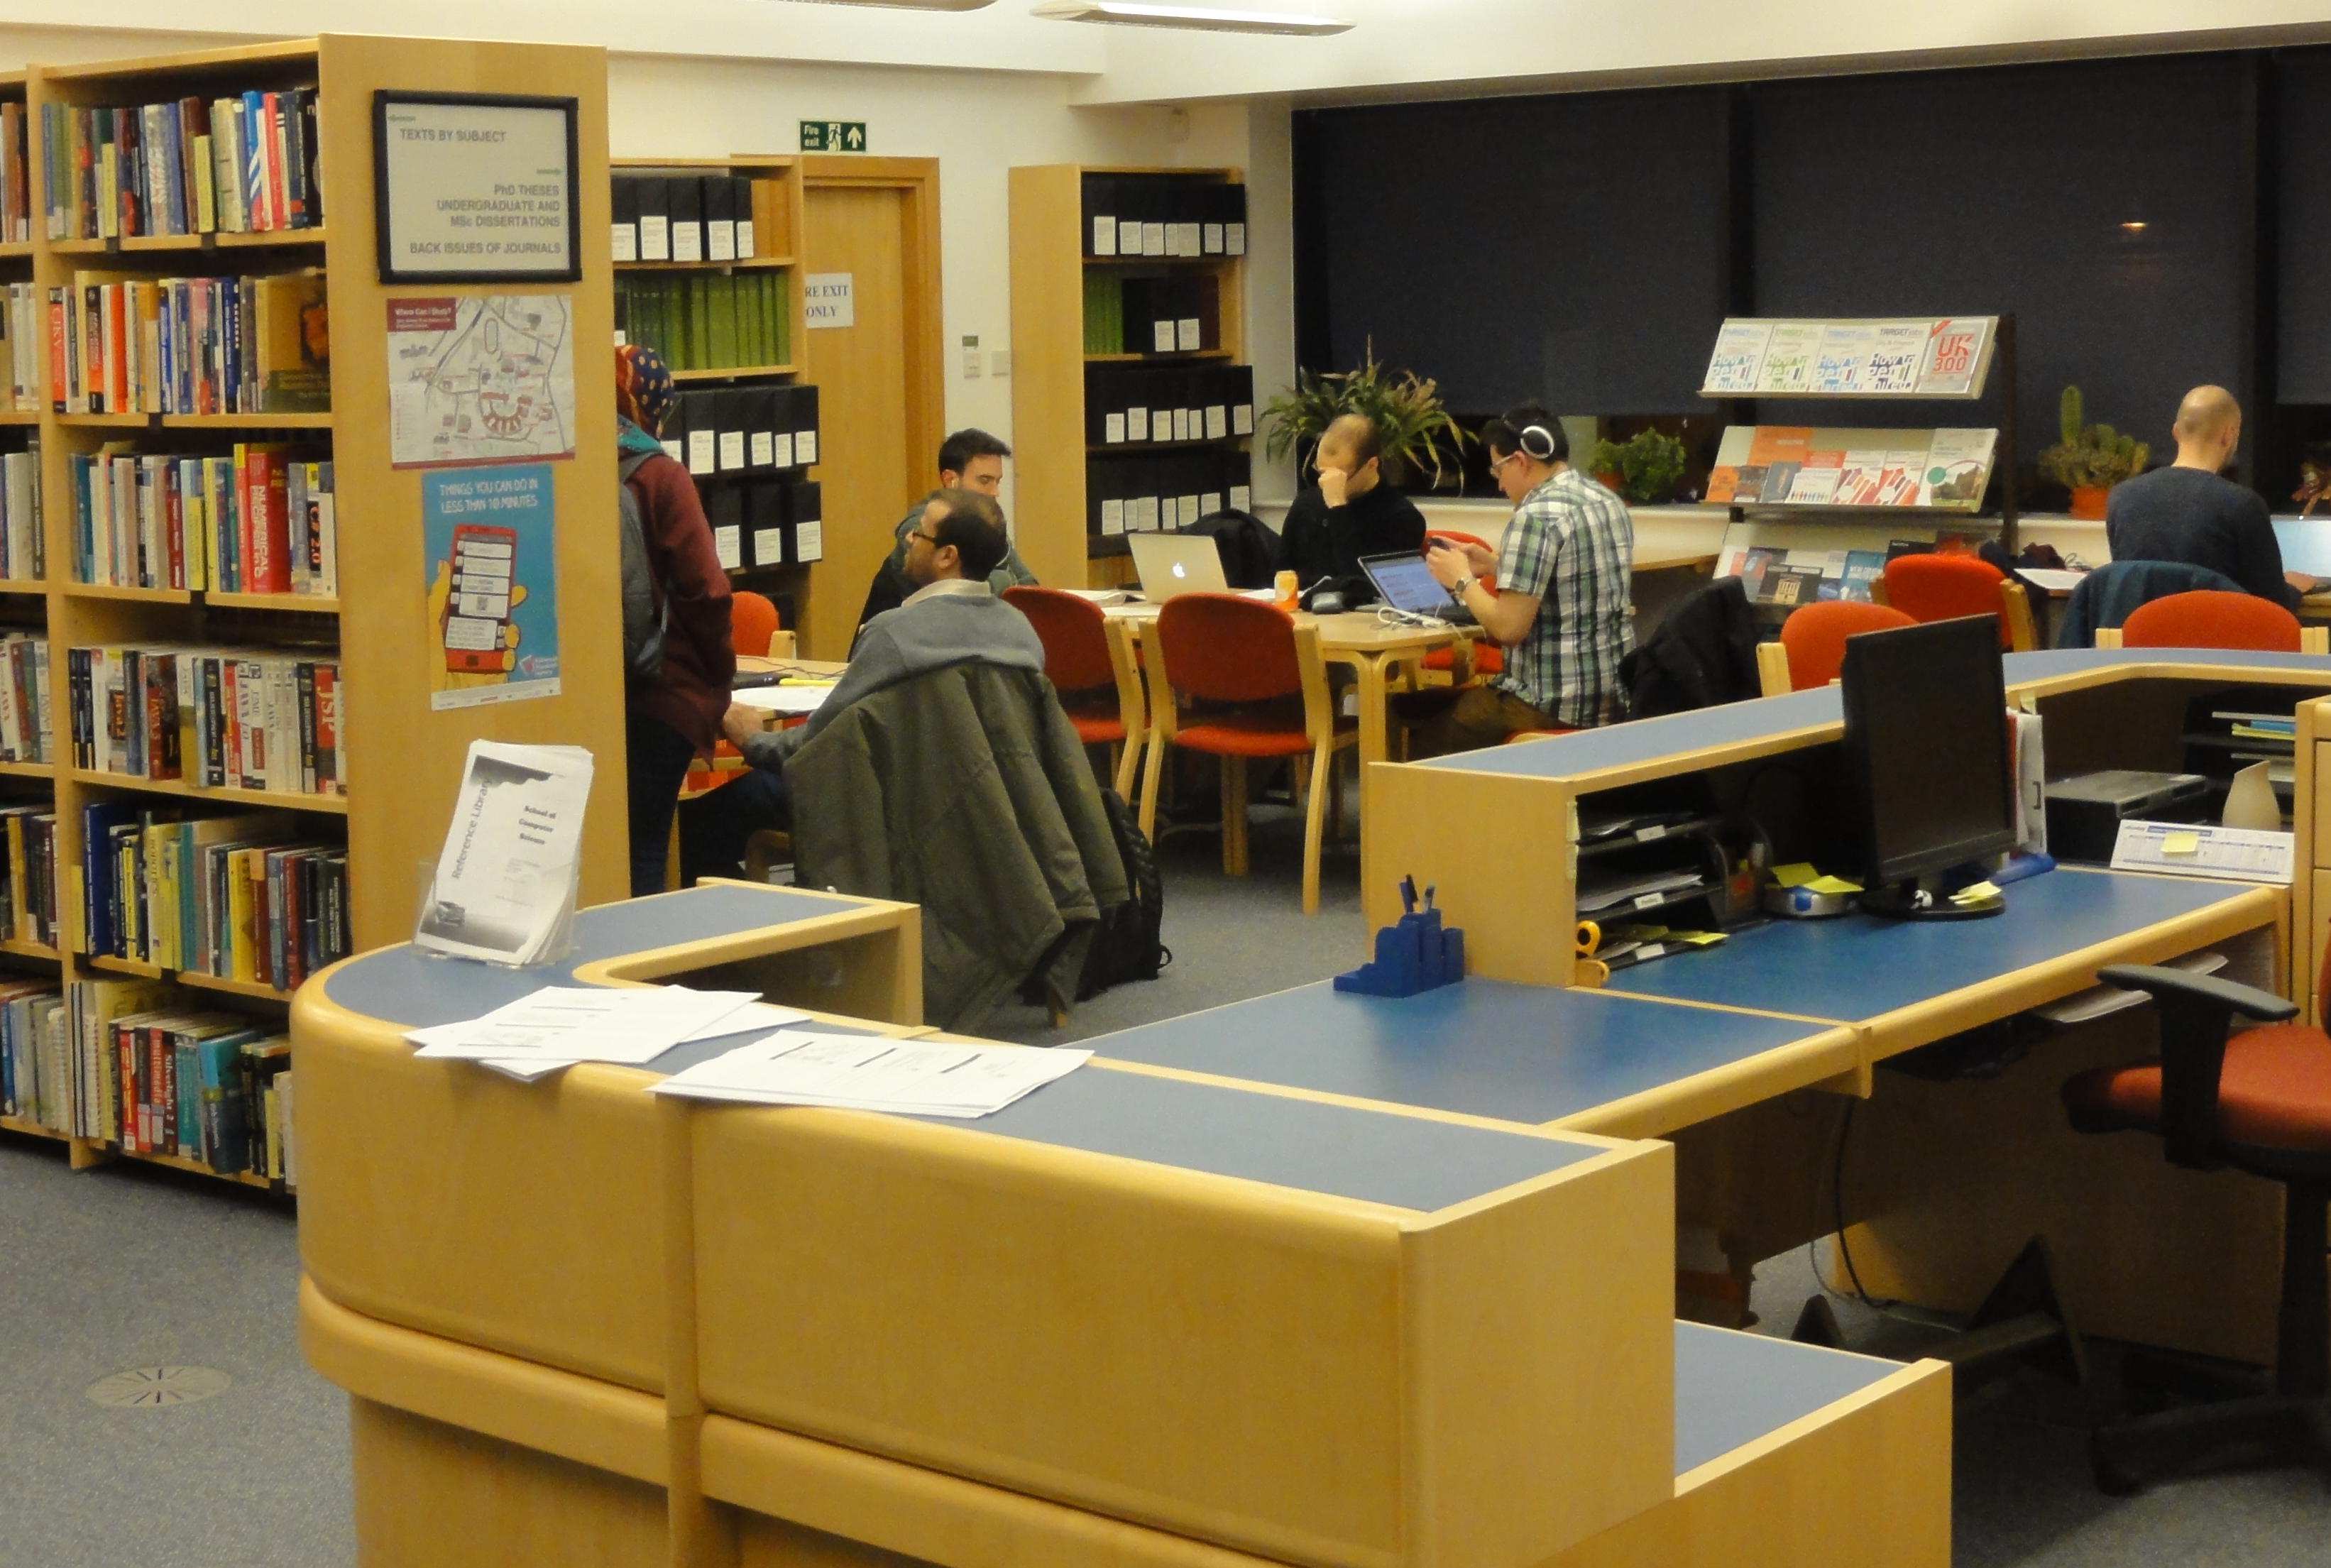
\includegraphics[width=2.5in]{fig/Library02.png}}\quad
  \subfloat[Semantic map of the library]{\includegraphics[width=2.5in]{fig/Library01.png}}\\
  \label{fig_library}\caption{The library setting}
\end{figure}

Because of the rules of the library and the nature of the location, the amount of activities is limited.
However, non-considered activities could eventually appear, as giving a greet, using a cellphone, talking, etc.
The amount of objects involved in the environment is also relatively small (books, tables, chairs, laptops, cabinets, etc.).

Our interest is to use this library setting as a test for activity recognition with a mobile robot, and moreover
The problem can be analysed with simple examples via simulation to build the core of a testing system, and later use real data and eventually a mobile robot.
%Libraries tend to share some similarities, there is the possibility to replicate the experiments from this work in other locations.
%This would create landmarks for testing and comparing different approaches, and direct the research towards a more general and better system.

%For the sake of simplicity and as a starting point, lets consider the following abstraction: a linear library (Fig. \ref{}).

%\begin{figure}[h]
%\centering
%\includegraphics[width=\textwidth]{fig/img_Aggarwal_Taxonomy2.pdf}
%\caption{The taxonomy of research in activity recognition described in \cite{Aggarwal11_HumanActivity}.}
%\label{fig:taxonomy}
%\end{figure}




%Some interesting activities to look at are:

%\begin{description}
%\item[book loan] A person goes to the reception with a book, spend some time on it and later leaves the library with the book.
%\item[book retrieval] A person arrives to the reception with a book and \textit{leaves} the book in the reception.
%\item[study] A person
%\end{description}


%TODO %TODO %TODO

\section{Document organization}

The rest of the document is organized in the following manner.

Chapter \ref{ch_relatedwork} presents related literature to the problem and discusses the results and limitations of previous approaches. The chapter starts with a brief historic presentation of perception in Artificial Intelligence and goes towards the problem of activity recognition. Section\ref{} presents a summary of how the problem of activity recognition has been treated before, and particularly regarding hierarchical description-based approaches, in which ASP is an alternative. In section \ref{sec_DBROB}, some previous works that integrate activity recognition and robotics are reviewed. Finally, in section \ref{sec_DBROB}, ASP is presented as an alternative for solving problems that require knowledge representation and reasoning.

Chapter \ref{ch_research_problem} presents the problem (section \ref{sec_problem}) and the proposed methodology (section \ref{sec_methodology}) to treat it. 

Chapter \ref{ch_eva} presents an experimental approach to evaluate the methodology proposed within this project. By using variations of the library setting environment (section \ref{sec_Library}), the problem can be studied gradually and the main components of an ASP-based approach can be remarked.

Chapter \ref{ch_wp} presents a work plan for the rest of the project duration (2 years) and proposes goals and tasks to achieve them. 

Finally, chapter \ref{ch_conc} presents the conclusions final comments regarding this project and about the developed ideas.









 % Intro & Motivation (Open areas proposed in the literatures)
% Outcome
%\chapter{Related Work}

% 0 - GENERALITIES
% Symbol ground
% Anchoring
% Frame Problem


% 1 - ACTIVITY RECOGNITION
% Historic origins
% Main branches
% Hierarchical pproaches


% 2 - ANSWER SET PROGRAMMING
% General background
% Related work to AR


% 3 - ASP + Robots -> ROSoClingo
% 
 % "Related Work" Literature rev (separated areas, in my case AR + ASP + KRR(incomplete) + Semantic Map)

%================================================
%================================================
%================================================
\chapter{Related Work}

% 0 - GENERALITIES
% Perception
% Symbol ground
% Anchoring
% Frame Problem

\section{Activity recognition}

Activity recognition is an important research area in the context of automated perception. 
It has many applications as surveillance, inspection, verification, generation of automated reports, etc. 
The main goal is to automatically analyse the ongoing activities from an unknown sensory source (a video sequence in most of the cases).
Activities play a relevant role in the interpretation of a scene, not only in physical terms, but also symbolically as they can usually be associated with a meaning or an interpretation.

The problem has been studied first in psychology. In \citep{Heider1944_Experimental}, an animation film was created using only polygons to demonstrate how the motion of abstract entities can be interpreted by a human observer.

The problem has been studied in AI from different areas, principally in computer vision or as a knowledge processing problem. 
Early work in computer vision can be traced back to the 1960-70s, as part of the effort to mimic human-like intelligence using visual perception components. In \citet{Johansson1973_VisualPer} locomotion of living organisms is studied using visual marks and then describes a study on interpretation of motion using visual dot markers mounted on a moving body, the patterns are described numerically, but also




The main difference between computer vision and image processing was a desire to recover the three-dimensional structure of the world from images, and to use this as a stepping stone towards full scene understanding \citep{Winston1975_PsyCV}. 


In the early 1970s, simple motion patterns of dots were studied to describe and recognize complex motion patterns (e.g. walking, shaking hands), \citep{Johansson1973_VisualPer}. 
Object recognition was treated in \citep{Barrow1971_RelatDesc} by decomposing an image in regions and describe the relations between them. 
Finally, in this decade, the \textit{block's world} problem was proposed as a test scenario for artificial intelligent systems, particularly regarding planning, knowledge representation and reasoning. 
One important characteristic of the problem is the requirement of a symbolic scene representation to do some reasoning. 
The block's world was also used with physical systems as the robot \textit{Shakey}, \citep{Nilsson84_Shakey}.





% COMPLETE - AR approaches (CV & KRR)
In the context of Artificial Intelligence it has been treated as a Computer Visioandverification, in aabout the problem of interpretation and understanding of a scene from sensory information and also using domain knowledge. 
It is mostly a perceptual action, however reasoning plays an important role too.

% Check the surveys to get the whole image



% 1 - ACTIVITY RECOGNITION PROBLEM
% Historic origins
% Approaches (camera, wearable device, ubiquitous computing)
% Main branches (single layer, multpiple layer)
% Hierarchical approaches

% 1.5 ACTIVITY RECOGNITION WITH A MOBILE ROBOT
A robot can be roughly conceived as a physical entity capable of sensing and performing actions in the world.
With this in mind, it seems clear that a robot, with sufficient sensing capabilities, is a good candidate to perform the task.


% 2 - ANSWER SET PROGRAMMING
% General background
% Related work to AR


% 3 - ASP + Robots -> ROSoClingo
% 
%================================================
%================================================
%================================================


%\chapter{Research Problem}

\section{Human activity analysis}
% Description of the problem

%TODO Main sentence for the problem

The application domain will dictate the activities to be recognized, the required precision, the sensors to be used and their location (environment located or wearable), the time constraints for deliberation,



%The main goal is to automatically analyse the ongoing activities from a sensory source (a video sequence in most of the cases).

%Activities can be understood in physical terms (space and time), but also symbolically as they can usually be associated with a meaning and a context. 

%Human activities are difficult to classify because they cover a broad range of situations and they depend on different parameters.
%Regarding their complexity, activities can be treated as hierarchical entities because high-level activities are usually composed of simpler actions.
Regarding the complexity of the activities, in \citep{Turaga2008_MaRecHuAcSurv}, two non-exclusive categories are used: actions and activities.
The first one is used for simple actions performed preferably by a individual, and activities are treated as a complex sequence of actions performed by several individuals. 
On a similar fashion, in \citep{Aggarwal11_HumanActivity}, a four layers categorization is proposed:

\begin{description}
\item[Gestures] Elementary movements of a person's body part, and are the atomic components describing a meaningful motion of a person. 
E.g. `stretching an arm', `raising a leg'.
\item[Actions] Single person activities that may be composed of multiple gestures organized temporally. 
E.g. `walking', `waving'.
\item[Interacions] Human activities that involve two or more persons and/or objects. 
E.g. `Two persons fighting', `a person eating an apple'.
\item[Group activities] The activities performed by conceptual groups of multiple persons and/or objects. 
E.g. `a football team playing a match', `a group of students making an exam'.
\end{description}









% Alternatives for each part
% > Observations
% > Knowledge (where? & how?, I'll do it by hand, but it's important to mention alternatives).
% > Representations
% *** CHECK THE orgnanization from the surveys
%   - Modelling activities in space (QSR)
%   - Modelling activities in time  (QSTR ~ Allen's, Fluent, Event, etc).
%   - Modelling activities semantically (Ontologies + Hierarchies)
% > Inference

% Test example

\section{Proposal} % Or alternatives

% Main parts of the problem

% A - Scene decomposition (locations, objects, persons)
%   > from observations to scene reconstruction

% B - 

% B - Representation 
% Modelling in space (QSR)
% Modelling in time (QSTR)
 % (Mike --> Model & Methodology) % Research Problem (Analysis) (Problem Definition -> Rafee)
%\input{040_Methodology.tex}% * Methodology (Here goes the strategy to face the problem, THE PROPOSAL!!)
%\chapter{Experimental Evaluation} % Or alternatives

Once presented the problem and a proposed model to treat it, some approach is required to test the feasibility of the ideas within this project.
With this in mind, and given the practical interest of the problem, an experimental methodology is proposed, using the library example from section \ref{sec_Library}, to gradually treat the problem and get closer to the applicability of the ideas in real situations.



%In this case, the proposed experimental environment is the library setting described in section \ref{sec_Library} with some simplifications and extensions to emphasize particular parts of the problem.
%By these means, the problem can be divided in smaller

\section{Library Example}

The library setting, presented in section \ref{sec_Library}, provides a good testing environment.
It has some desired qualities for experimentation, principally, a bounded space and a compact set of activities.
%Now, some incremental












If we reuse the library example from chapter 1, it would be worthy to show how the presented approach applies to that problem.
With this in mind, let's first make a simplification of the example.

In Figure \ref{fig:ex_library} is presented a \textit{linear} library. 
It has five connected and consecutive regions: (A) main entrance, (B) printing area, (C) reception, (D) bookshelf and (E) common area.
In this simplified world a person and a robot can move linearly to any region, and they don't obstruct each other.
An activity is performed by a person by visiting regions in a proper order and spending \textit{enough} time on each of them, these intervals are considered within the activity representation.
The challenge here is to recognize the activities of the person

\begin{figure}[h]
\centering
\includegraphics[width=\textwidth]{fig/ex_library.pdf}
\caption{Sensing will be targeting relevant features from humans, objects and from the environment.}
\label{fig:ex_library}
\end{figure}

Some extensions can be induced to this simple world.
\begin{itemize}
\item A robot can have limited sensors, so it will only be able to sense two regions at the same time. 
So, some activeness is required. For example, being observed a person going towards the common area, the robot can move to confirm the position of the person.
\item Handling multiple subjects in the scene, complicates the problem. The robot won't be able to observe all of them, but may try to maximize the observations and after labelling some individuals may go back and sense the rest of the subjects.
\item Object recognition can be induced to disambiguate activities. For example, two activities with the same region description can have an additional parameter regarding the presence of an object. In these cases, a robot can go an confirm the presence or absence of the object to discriminate its hypotheses. 
\end{itemize} 


However, let's use now just the simple case with only one subject and with the activities defined just regarding the visited regions.
The following activities can be defined:

\begin{description}
\item[print]$B$ 
\item[study]$D \rightarrow E$
\item[bookLoan]$D \rightarrow C$
\item[bookRetrieval]$C$
\item[requestAssistance]$C$
\end{description}

%TODO %TODO %TODO Complete the example.







\section{Final evaluation}

First, this project makes emphasis in the use of a robot, which has some evident limitations.
Sensors are constrained to defined ranges and the thrown data usually presents noise.
Actuators also present inaccuracies and time-delayed responses.
Processing capabilities are also limited in a robot, so the amount of data collected with a robot should be minimized and processed efficiently whenever is possible.
%This is, however, the current state in robotics and this is considered by considering sensor models, 

Regarding ASP, here is used for knowledge representation and reasoning purposes. 
It can also provide a path to plan actions for the robot.
ASP should be used with reserve as it is used to model combinatorial NP-hard problems.
With this in mind, should be noted that ASP implementations are limited in efficiency and the modelled problems can grow very easily.
This is considered in this project by restricting the domain application (to a library), the amount and granularity of the descriptions for activities, objects and places. 

The idea is to go from a simple case to more complex, general and realistic cases. 
An experimental approach is going to be followed, so it an important question how are the results going to be evaluated.
Two possibilities are considered now.

First, to compare our library setting with other techniques. 
This is, to implement other approach, run it in the same conditions than the one developed in this project, and compare results.
This have the advantage than the experiments can be in control and many situations can be explored (e.g. different starting points, different environmental conditions, different activities, objects, etc.).

The second possibility is to use a dataset for activity recognition, as \citep{Tenorth2009_TUMKData}, and compare our ASP-based approach with other ones.
This has the advantage that the results to compare are already available as well as the sensory data.
However, the disadvantage is that there are no datasets for activity recognition with robots. 
So the way to proceed would be only to compare the stand-alone activity recognition system with ASP.



% Main parts of the problem

% A - Scene decomposition (locations, objects, persons)
%   > from observations to scene reconstruction

% B - 

% B - Representation 
% Modelling in space (QSR)
% Modelling in time (QSTR)











% Evaluation (Pros + Cons, Possible failures, etc.)
%\chapter{Work Plan}\label{ch_wp}

The main goal of this project is to present a concise study of the integration of ASP and robotics to treat the problem of activity recognition.
By this mean, a work plan should be submitted as a guide line to direct future activities and to measure the progress in the the project. In the following section a plan is presented for the next 2 years. The proposed work plan has been created considering three classes of goals: project goals, research goals and academic responsibilities.

First \textit{project goals} are those which moves forward the research project. 
As the direction of research is now clear (ASP-based activity recognition with a mobile robot), and the literature review is considerably up to date, these goals are in the sense of the implementation, testing and analysis of the proposed methodology, to find the paths that conduce to better results. 
At the beginning these tasks will be simple and look to proof the feasibility of the proposed ideas. 
In the final stages, the tasks will be driving the project towards more realistic cases and/or towards specific problems that proof to be relevant.

\textit{Research goals} are those which serve for research training purposes and those enable the participation of the current project in activities within the research community, e.g. conferences, research school meetings, presentations, academic writing, etc.

Finally, \textit{academic responsibilities} are conformed with those tasks that are mandatory for PhD students within an academic program.

\section{Work Distribution}

\subsection*{T01 - Terminal Simulation}
\paragraph{Objectives}
\begin{itemize}
\item Start the implementation of an activity recognition system using the 2D library setting.
\item Explore simple representations of activities.
\item Get familiar with ASP tools (Clingo, ROSoClingo).
\end{itemize}
\paragraph{Tasks}
\begin{enumerate}[label= T01-\Alph*:]
\item The implementation of a simple (terminal) activity recognition system using ASP tools (potassco).
\item Test different representations of activities based on the interaction between spaces (regions) and humans (positions).
\item Test sequential representation of activities, i.e. a human visiting different locations.
\item Consider objects in scene and within the activity representations.
%\item \textit{Optional} Add visualisation software, e.g. NetLogo.
%\item \textit{Optional} Consider simple robot activity.
\end{enumerate}


\subsection*{T02 - MORSE Simulation}
\paragraph{Objectives}
\begin{itemize}
\item Implement a more realistic 3D simulation of the library setting.
\item Integrate ROS, Potassco and MORSE in a system.
\item Extend the representations of activities to a 3D environment; i.e. start considering geometrical entities as regions, trajectories, etc.
\end{itemize}
\paragraph{Tasks}
\begin{enumerate}[label= T02-\Alph*:]
\item Create the library setting in MORSE and attach one robot to the environment.
\item Integrate ROS and Potassco (via ROSoClingo) with the MORSE simulation.
\item Create interfaces, in ROS, to extract and describe important spatial entities as regions, trajectories, etc.
\item Extend the representation of activities for a 3D environment.
\end{enumerate}


\subsection*{T03 - Qualitative description}
\paragraph{Objectives}
\begin{itemize}
\item Implement qualitative spatial representations between the entities on scene.
\item Implement qualitative temporal representations between events.
\item Enable the representations of activities to use QSTR.
\end{itemize}
\paragraph{Tasks}
\begin{enumerate}[label= T03-\Alph*:]
\item Implement RCC and QTC, use regions in the map, human bounding boxes, human trajectories, objects bounding boxes, etc.
\item Implement Allen's Interval Algebra between events. 
\item Enable and expand the representation of activities to integrate QSTR\footnote{The desired goal would be to have only qualitative representations. However, a proper balance between qualitative and quantitative approaches is an important topic to study more carefully.}.
\end{enumerate}

\subsection*{T04 - Knowledge Base}
\paragraph{Objectives}
\begin{itemize}
\item Integrate a knowledge base from different sources, e.g. activity representations, semantic maps, ontologies, online knowledge sources, etc.
\end{itemize}
\paragraph{Tasks}
\begin{enumerate}[label= T04-\Alph*:]
\item Implement a Knowledge Base from different sources with the capacity to be gradually enlarged and consulted via ASP. The minimum integration would consider the activity representations and the semantic maps.
\item Implement the proper consult mechanisms via ASP.
\item Implement a \textit{reporting} module to analyse the conclusions of the activity recognition system (ASP) to \textbf{report missing data}. Is important for the system to be aware of which data is missing and also, which part of it is more relevant to get more confident results.
\item Explore the capacity to generate new rules from experience.s
\end{enumerate}

\subsection*{T05 - Semantic Mapping}
\paragraph{Objectives}
\begin{itemize}
\item Implement semantic mapping of activities within the system.
\item Spatial and temporal analysis.
\end{itemize}
\paragraph{Tasks}
\begin{enumerate}[label= T05-\Alph*:]
\item Extract relevant features from the environment, e.g. objects, humans and entities from the environment (regions, corridors, doors, etc.). First, at the simulation stage this can be done by explicitly getting this information, then later this can be done using markers, and finally by using non-invasive sensing methods.
\item Implement the capacity to make maps of activities. Static maps first and then dynamic ones.
\item Integrate pattern recognition techniques to the generation of maps.
\item Integrate the semantic maps into the Knowledge Base and implement mechanisms to generate ASP rules from it.
\end{enumerate}

\subsection*{T06 - Active Perception}
\paragraph{Objectives}
\begin{itemize}
\item Restrict the perception of the robot and implement active strategies (planning, control) to improve the activity recognition process with the mobile robot.
\end{itemize}
\paragraph{Tasks}
\begin{enumerate}[label= T06-\Alph*:]
\item Implement plans of action for the robot, e.g. maximize surface coverage, maximize human sensing data collection, look for specific data in the environment (missing data), etc.
\item Design experiments (simulated scene) and compare the designed active strategies.
\end{enumerate}

\subsection*{T07 - Real data collection and testing of the ASP-based activity recognition system}
\paragraph{Objectives}
\begin{itemize}
\item Collect real data, and or use standard datasets for activity recognition system.
\item Use this data to compare the proposed ASP-based activity recognition with other state-of-the-art approaches.
\end{itemize}
\paragraph{Tasks}
\begin{enumerate}[label= T07-\Alph*:]
\item Get real data to analyse. This can be done by using standard datasets \citep{Tenorth2009_TUMKData,Liu2011_BenchmarkDatasHAR}, by using collected data from the project STRANDS \citep{Hawes2013_STRANDS} or by collecting it from a controlled environment.
\item Integrate a ROS based system to be able to use the collected data, particularly, proper object recognition and human sensing techniques.
\item Analysis and comparison of the results.
\end{enumerate}

\subsection*{T08 - Robot testing}
\paragraph{Objectives}
\begin{itemize}
\item Test the activity recognition system with a robot in a real environment and with an active participation of it.
\end{itemize}
\paragraph{Tasks}
\begin{enumerate}[label= T08-\Alph*:]
\item Design experiments to run.
\item Integrate system within a robotic platform. 
\item Run experiments.
\item Analysis.
\end{enumerate}

\subsection*{T09 - Reporting progress and results}
\paragraph{Objectives}
\begin{itemize}
\item Report the advances within the project.
\item Research training in writing and oral presentation.
\end{itemize}
\paragraph{Tasks}
\begin{enumerate}[label= T09-\Alph*:]
\item Write RSMG reports and prepare thesis group meetings.
\item Participation in activities in the University to present the project.
\item Write thesis.
\end{enumerate}

\subsection*{T10 - Publishing, Conferences and Workshops}
\paragraph{Objectives}
\begin{itemize}
\item Present results to the research community.
\item Submit work for external judgement and receive feedback.
\item Interact with other researchers in the field.
\item Research training in academic writing, oral presentation.
\end{itemize}
\paragraph{Tasks}
\begin{enumerate}[label= T10-\Alph*:]
\item Prepare and submit work in top conferences in the area (\textit{Goal: Get work accepted for two conferences.}).
\begin{itemize}
\item ICRA - International Conference on Robotics and Automation
\item IROS - International Conference on Intelligent Robots and Systems 
\item AAAI - National Conference on Artificial Intelligence
\item IJCAI - International Joint Conference on Artificial Intelligence
\item RSS - Robotics Science and Systems
\item SMC - IEEE International Conference on Systems, Man, and Cybernetics
\item LPNMR - Logic Programming and Non-monotonic Reasoning
\end{itemize}
\item Prepare and submit work for a top journal in the area (\textit{Goal: Get one article accepted for publication}).
\begin{itemize}
\item International Journal of Robotics Research (IJRR)
\item IEEE Transactions on Robotics (TRO)
\item IEEE Robotics and Automation Magazine (RAM)
\item Autonomous Robots (AURO)
\item Robotics and Autonomous Systems
\item Journal of Intelligent & Robotic Systems
\end{itemize}
\end{enumerate}


\section{Time table}

The proposed time table is shown in Fig. \ref{fig_gantt}.


\begin{landscape}

\begin{figure}[ftbp]
\begin{center}

\begin{ganttchart}[hgrid,
%vgrid={*1{blue, ultra thick}, dotted},
vgrid,
x unit=7mm, y unit title=7mm, y unit chart=7mm, bar/.style={fill=gray!50},
incomplete/.style={fill=white},
progress label text={},
bar height=0.7,time slot format=isodate, compress calendar]{2015-04-01}{2017-06-31}
\gantttitlecalendar{year, month} \\
%\gantttitlecalendar{year, month } \\
%\ganttgroup{Absences}{2015-04-02}{2015-04-06} \\
\ganttbar{T01}{2015-04-01}{2015-04-30}\\ % Terminal simulation
\ganttbar{T02}{2015-05-01}{2015-06-30}\\ % MORSE simulation
\ganttbar{T03}{2015-07-01}{2015-07-30}\\ % Qualitative description
\ganttbar{T04}{2015-08-01}{2015-10-31}\\ % Knowledge Base
\ganttbar{T05}{2015-09-01}{2015-11-31}\\ % Semantic Mapping
\ganttbar{T06}{2015-12-01}{2016-02-29}\\ % Active Perception
\ganttbar{T07}{2016-03-01}{2016-06-30}\\ % Real data 
\ganttbar{T08}{2016-07-01}{2016-10-30}\\ % Robot testing
\ganttbar{T09}{2016-11-01}{2017-04-30}\\ % Reporting Progress
\ganttmilestone{RSMG}{2015-05-01}
\ganttmilestone{}{2015-11-01}
\ganttmilestone{}{2016-05-01}
\ganttmilestone{}{2016-11-01}
\ganttmilestone{}{2017-05-01}
\\
\ganttbar{T10}{2015-11-01}{2015-12-31}   % Conferences
\ganttbar{T10}{2017-01-01}{2017-02-28}
\ganttbar{T10}{2016-06-01}{2016-07-30}
\end{ganttchart}


\end{center}
\caption{Long-term time table} \label{fig_gantt}
\end{figure}

\end{landscape}








% * Work Plan (Research Goals+- --> Paul Engelfield)
% Work Done (so far)
% Timetable

% MAke a Timeline of AR
% Check "Paul Engelfield" --> Good Report

% *5min sketch of the report at the begining

% Bibliography
\clearpage
\bibliographystyle{abbrvnat}
\bibliography{/home/kilgore/Dropbox/Public/Docs/mabp_bibliography.bib}
%\bibliography{Bibliography.bib}


\end{document}
